\section{Factor-Separated Evaluation Results}
\label{sec:factor_results}

All 270 scheduled evaluations completed. Table~\ref{tab:factor_overall}
summarizes the two 135-run arms. The adaptive method increases compound pass from
85 to 100 and strict tracking pass by the same amount. The paired difference
is 11.11 percentage points with a block- and seed-aware 95\% bootstrap
interval of [3.70, 18.52]. Mean MRE and NRMSE decrease by 1.83 and 1.28
percentage points, respectively; both intervals exclude zero. Mean planning
samples decrease by 7.97 and mean median planning time by 25.65~ms.

\begin{table}[t]
\centering
\caption{Factor-separated evaluation over 135 runs per planner.}
\label{tab:factor_overall}
\small
\begin{tabular}{lrr}
\toprule
Outcome & Fixed & Adaptive \\
\midrule
Task success & 133 & 132 \\
Tracking pass & 85 & 100 \\
Compound pass & 85 & 100 \\
Mean MRE (\%) & 12.16 & 10.33 \\
Mean NRMSE (\%) & 15.07 & 13.78 \\
Samples $>15$~N & 2 & 2 \\
Maximum peak (N) & 17.399 & 17.905 \\
Planning samples & 128.0 & 120.0 \\
Median time (ms) & 101.09 & 75.43 \\
\bottomrule
\end{tabular}
\end{table}

The benefit is a tracking--computation trade-off rather than a general safety
gain. Task success changes by $-0.74$ percentage points, interval
$[-4.44,0.00]$, and sampled-limit violations remain two in each arm. Mean peak
force increases by 0.247~N, interval $[0.045,0.428]$~N. At 12~N, tracking
improves from 5/45 to 17/45, but task success changes from 43/45 to 42/45.

Figure~\ref{fig:factor_results} shows that the aggregate improvement is not
uniform. Compound pass rises for the incline, both paths, both friction levels,
both support stiffnesses, and the reference block. On the cylinder it falls
from 7/15 to 6/15. The cylinder also contains every task failure and sampled
force-limit violation: its maximum peak is 17.399~N for the fixed planner and
17.905~N for the adaptive planner. The method therefore improves regulation
under most isolated shifts but does not resolve weak curvature combined with
a 12~N target.

For comparator context, an earlier matched simulation suite used the same
Cartesian action interface. The original direct PPO configuration achieved
0/90 task completions, while the fixed TD-MPC2 planner and actor-only control
achieved 19/90 and 18/90 compound passes.
Adaptive admittance achieved 11/18 compound passes and was strongest at 5 and
8~N but degraded at 12~N. The admittance values are one deterministic run per
cell and do not enter the paired interval analysis. For the fixed-planner
versus actor-only comparison, task and tracking differences were 2.22 and
3.33 percentage points, with intervals $[-6.67,13.33]$ and
$[-4.44,13.33]$. The design therefore resolved neither a benefit nor
equivalence for the historical online planner. These results establish
learned and structured-control references; the paired M1--M4 experiment above
isolates the contribution of regime adaptation.

The expanded PPO study covers three budgets and six one-factor variants over
five seeds. The development rule selected clip ratio 0.1 at 165,548
transitions per seed, with 3/90 compound and 11/90 task passes. On the two
confirmation suites, that endpoint achieved 0/90 task and compound passes on
the matched weak-curvature set, followed by 19/135 task and 6/135 compound
passes on the factor-separated set. All six compound passes came from one
seed. By comparison, RA-RMPPI achieved 100/135 compound passes on the same
factor-separated cells. This cross-family contrast is descriptive because
the checkpoint seeds are independent; it is not included in the paired
M1--M4 interval. The Supplementary Material reports every PPO
endpoint. The result shows that the weak PPO reference persisted across the
tested budget and local hyperparameter range, without making an
algorithm-independent claim about PPO.

The original PPO training record provides the matched-budget anchor. Across
645 training episodes, 3 completed the task and 470 contained a sampled
force-limit violation. Figure~\ref{fig:ppo_training} shows that training
reduced the violation rate but did not produce reliable task completion at
82,774 transitions per seed.

\begin{figure*}[t]
\centering
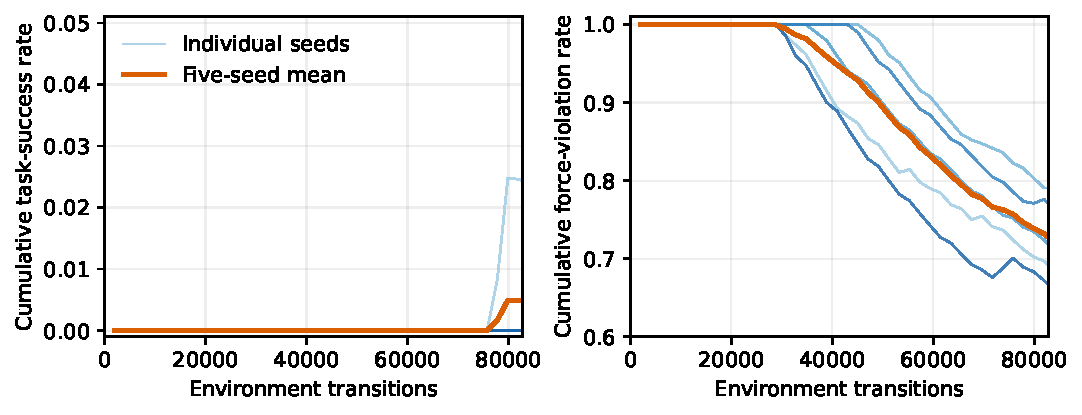
\includegraphics[width=0.92\textwidth]{figures/ppo_training_curves.pdf}
\caption{Original matched-budget direct PPO training over five seeds and
82,774 environment transitions per seed.}
\label{fig:ppo_training}
\end{figure*}

\begin{figure*}[t]
\centering
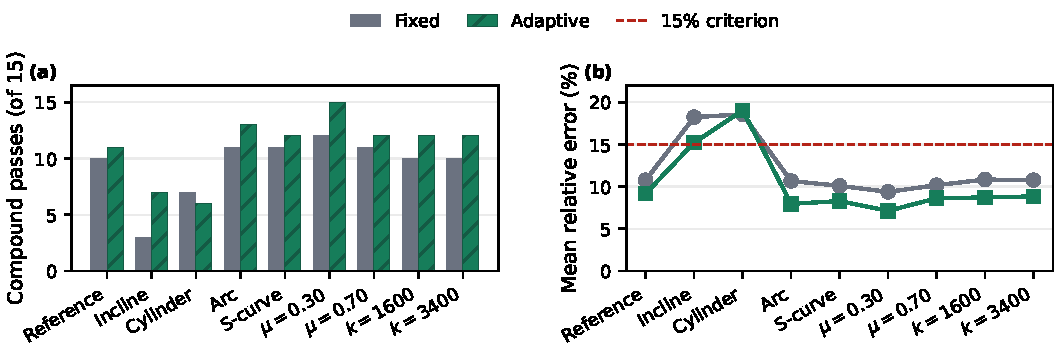
\includegraphics[width=0.96\textwidth]{figures/factor_separated_results.pdf}
\caption{Factor-separated task-and-tracking outcome and mean force error;
15 evaluations per factor level and planner.}
\label{fig:factor_results}
\end{figure*}
